\chapter{Исследовательская часть}

В данном разделе будет проведен сравнительный анализ алгоритмов по времени выполнения в зависимости от количества матриц и их размеров.

\section{Технические характеристики устройства}

Тестирование проводилось на устройстве со следующими техническими характеристиками:

\begin{itemize}[label=---]
	\item операционная система Window 10 Home Single Language;
	\item память 8 Гб;
	\item процессор 11th Gen Intel(R) Core(TM) i7-1165G7 2.80 ГГц, 4 ядра.
\end{itemize}

\section{Демонстрация работы программы}

На рис. \ref{fig:test_parallel} представлена демонстрация работы программы.

\begin{figure}[h]
	\centering
	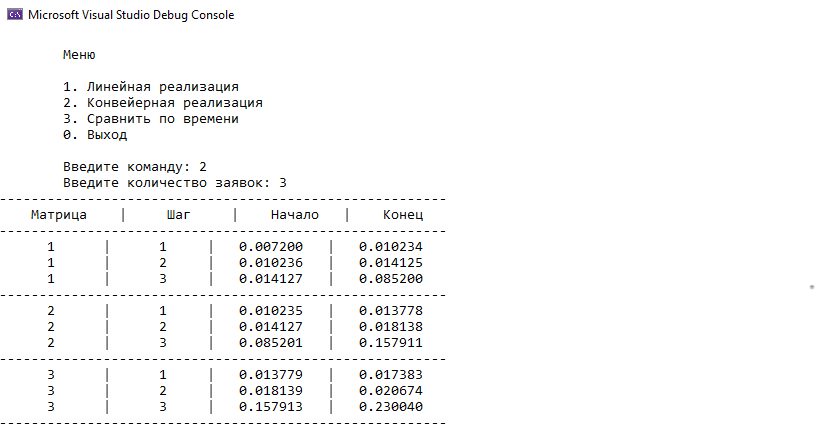
\includegraphics[scale=0.9]{img/exp2.png}
	\caption{Демонстрация работы программы при конвейерной обработки данных}
	\label{fig:test_parallel}
\end{figure} 

\section{Время выполнения алгоритмов}

Результаты замеров времени работы алгоритмов обработки матриц для конвейерной и ленейной реализаций представлены на рисунках \ref{img:graph_diff_quantities} -- \ref{img:graph_diff_sizes}. Замеры времени проводились в секундах и усреднялись для каждого набора одинаковых экспериментов.

% \imgScale{1}{time}{Замеры времени работы алгоритмов для конвейерной и ленейной реализаций}

\imgScale{0.5}{graph_diff_quantities}{Зависимость времени работы алгоритмов от кол-ва матриц (размеры матриц 100х100)}

\imgScale{0.5}{graph_diff_sizes}{Зависимость времени работы алгоритмов от размера матриц (кол-во матриц = 100)}

\clearpage

\section{Вывод}

В этом разделе были указаны технические характеристики машины, на которой происходило сравнение времени работы алгоритмов обработки матриц для конвейерной и ленейной реализаций.

В результате замеров времени было установлено, что конвейерная реализация обработки лучше линейной
при большом кол-ве матриц (в 2.5 раза при 400 матрицах, в 2.6 раза при 800 и в 2.7 при 1600). Так же конвейерная обработка показала себя лучше при увеличении размеров обрабатываемых матриц (в 2.8 раза при размере матриц 160х160, в 2.9 раза при размере 320х320 и в 2.9 раза при матрицах 640х640). Значит при большом кол-ве обрабатываемых матриц, а так же при матрицах большого размера стоит использовать конвейерную реализацию обработки, а не линейную.


